\documentclass{article}

% if you need to pass options to natbib, use, e.g.:
% \PassOptionsToPackage{numbers, compress}{natbib}
% before loading nips_2016
%
% to avoid loading the natbib package, add option nonatbib:
% \usepackage[nonatbib]{nips_2016}

\usepackage[final]{nips_2016}

\usepackage{amsmath} % used for matrices in math mode

% to compile a camera-ready version, add the [final] option, e.g.:
% \usepackage[final]{nips_2016}

\usepackage[utf8]{inputenc} % allow utf-8 input
\usepackage[T1]{fontenc}    % use 8-bit T1 fonts
\usepackage{hyperref}       % hyperlinks
\usepackage{url}            % simple URL typesetting
\usepackage{booktabs}       % professional-quality tables
\usepackage{amsfonts}       % blackboard math symbols
\usepackage{nicefrac}       % compact symbols for 1/2, etc.
\usepackage{microtype}      % microtypography
\usepackage{textcomp}

\usepackage{graphicx}  % Required for including images
\usepackage{verbatimbox}


\usepackage{subcaption}
\captionsetup{compatibility=false}

\bibliographystyle{dcu}

\title{Pre-Training CNN's Using Convolutional Autoencoders}

% The \author macro works with any number of authors. There are two
% commands used to separate the names and addresses of multiple
% authors: \And and \AND.
%
% Using \And between authors leaves it to LaTeX to determine where to
% break the lines. Using \AND forces a line break at that point. So,
% if LaTeX puts 3 of 4 authors names on the first line, and the last
% on the second line, try using \AND instead of \And before the third
% author name.

\author{
  Maximilian~Kohlbrenner\\
  TU Berlin\\
  \texttt{mail} \\
  \And
  Russell Hofmann\\
  TU Berlin\\
  \texttt{r.hofmann@campus.tu-berlin.de} \\
  \AND
  Sabbir Ahmmed \\
  TU Berlin \\
  \texttt{mail}\\
  \And
  Youssef Kashef \\
  TU Berlin \\
  %% Address \\
  \texttt{mail}
  %% \And
  %% Coauthor \\
  %% Affiliation \\
  %% Address \\
  %% \texttt{email} \\
}

\begin{document}
% \nipsfinalcopy is no longer used

\maketitle

\begin{abstract}
  We are comparing the effect of pretraining.
\end{abstract}


\section{Introduction}
  % CNN SOTA but difficult to train (local minima)
  While deep convolutional neural networks have attained state of the art performance in many computer vision tasks, their training still remains a difficult task and results are highly dependend on the model initialization (local minima). 
  % classification learns: representation + decision
  During a classification task, a CNN first learns a new data representation using its convolution layers as feature extractors and then uses several fully-connected layers for decision-making. 
  % representation might be more general
  While the representation after the convolutional layers is optizimed for classification, some learned features might be more general and also useful outside of this specific task. 
  Instead of directly optimizing for classification, one can therefore as well begin with focussing on the learned representation before starting to work on the classification problem.
  % representation learning: autoencoder
  One possible way to do this uses a convolutional autoencoder, an unsupervised method that allows to train the convolutional layers independently from a classification task to learn a new data representation. 
  % weight transfer
  The learned weights can then be used as a starting point to initialize a convolutional neural networks convolution layers. 
  % small datasets: needs to learn both at the same time
  This becomes of special interest when only very few labeled examples are available since additional, unlabeled datapoints can be used for the representation learning task. 
  % reference paper (it worked)
  \citep{masci2011stacked} showed that pre-training a neural network using autoencoder weights can improve the classification accuracy consistently by a small margin.\footnote{In their paper, pre-training boosted the classification accuracy by up to 3.2\% (on \emph{CIFAR-10} restricted to 1k training datapoints.)}
  % We verify those results on the MNIST + CIFAR-10 benchmarks
  We reproduce these results on the common \emph{MNIST} \citep{lecun1998mnist} and \emph{CIFAR-10} \citep{krizhevsky2009learning} benchmarks and finally demonstrate that the approach can be used very effectively on the \emph{Extended Cohn-Kanade} \citep{kanade2000comprehensive,lucey2010extended} dataset where label information is not only extemely sparse but also ambiguous. 
  % We demonstrate the use of pre-training on the CK+ dataset where only very few correctly datapoints are available and show that the additional, non-labeled datapoints can be used to obtain a better classification accuracy.

\section{Related Work}
Erhan et al. \citep{Erhan10} showed that unsupervised pre-training adds robustness to a deep architecture and pre-trained networks give consistently better
generalization. They also suggested that increasing the depth of an architecture that is not pre-trained increases the probability of finding poor apparent local minima. They observed that pre-trained networks learn qualitatively different features compared to networks without pre-training. Pre-training not only gives a good initial
marginal distribution but also captures more intricate dependencies between parameters. Another interesting point which they asserted is that unsupervised pre-training exhibits some properties of a regularizer and classical regularization techniques (e.g L1/L2) do not achieve
the same performance as unsupervised pre-training. A point of caution, however, is the fact that the pre-trained models obtain worse training errors, but better generalization performance when the layers are big enough in deep architectures.

Masci et al. \citep{masci2011stacked} introduced the Convolutional Auto-Encoder (CAE), an unsupervised method for hierarchical feature extraction, which learns biologically plausible filters. Masci et. al demonstrated that a CNN can be initialized by a CAE stack. Although CAE’s overcomplete hidden representation makes learning harder than the standard auto-encoder,  interesting and visually nicest filters emerge if a max-pooling layer is used. They experimented with 20 7x7 filters of 4 CAEs of the same topology trained as follows on MNIST dataset- (i) the first one on original digits, (ii) the second one on noisy inputs with 50\% binomial noise added,
(iii) the third one with an additional max-pooling layer of size 2x2,
(iv) the fourth one on noisy (30\% binomial noise) inputs with a max-pooling layer of size 2x2.
When they compared the results, it turned out that interesting and biologically plausible filters emerged only when the CAE had been trained with a max-pooling layer. When the CAE was trained without any additional constraints, it learned trivial solutions and when they trained the CAE with additional noise, it became more localized. They repeated the above experiments on CIFAR10 dataset and found striking impact of a max-pooling layer whereas adding noise had almost no visual effect except on the weight magnitudes, indicating that max-pooling is essential. They also demonstrated that pre-trained CNNs consistently outperform randomly initialized CNN.

Makhzani et al. \citep{Makhzani14} explored combining the benefits of convolutional architectures and autoencoders for learning deep representations in an unsupervised manner. They proposed an unsupervised learning algorithm for training CAE with a very strong sparsity constraint on the activity within each feature map. To achieve that they trained a CAE layer by layer on MNIST, CIFAR-10 and NORB datasets, where in each layer sparsity was achieved using a winner-take-all activation function within each feature map.  The sparse convolutional autoencoder was based on a CAE with a ReLU activation function.

Khorrami et al. \citep{Khorrami17} achieved state-of-the-art performance on two face expression recognition
benchmarks: the extended Cohn-Kanade (CK+) dataset
and the Toronto Face Dataset (TFD) by training a zero-bias CNN on facial expression data and by introducing an approach to decipher which portions of the face influence the CNN’s predictions.

Hamester et al. \citep{hamester15} proposed a model for face expression recognition based on a variant of the Multi-channel Convolutional Neural Network (MCCNN) earlier introduced by \cite{Barros14} which does not depend on any hand-crafted or task specific feature extraction but exploits unsupervised learning, using a multiple CNNs based 2-channel architecture, where the CNNs first process information independently and then all streams merge in a fully connected layer, which is used for classification. The wights of the channel are trained in an unsupervised fashion as a convolutional auto-encoder (CAE). They evaluated the model on JAFFE dataset and found that the model is a very viable method for facial expression recognition. They easily reached the state-of-the-art recognition rates with minimal effort and achieved an average of 95.8\% accuracy which was almost 3\% and 8\% higher than the other state-of-the-art methods (Sobel-based filters and McFIS method) used by \citep{Subramanian12}.

\subsection{Datasets}
  In previous work \citep{masci2011stacked}, the authors applied the approach of pre-training by a convolutional autoencoder to two standard image classification datasets, MNIST and CIFAR-10.
  Since one part of our project consists of reproducing these results, we will shortly introduce both these datasets here.
  \subsubsection{MNIST}
    MNIST \citep{lecun1998mnist} is the standard dataset used for image classification. It consists of scanned handwritten digits, which are 28 by 28 pixel grayscale images. As they are digits, the goal is to classify the correct one of 10 classes.
    The dataset consists of 55000 training, 5000 validation, and 10000 test images.
  \subsubsection{CIFAR-10}
    The CIFAR dataset \citep{krizhevsky2009learning} is made out of natural scenes, which are 32x32 colorized images. The relatively low resolution, while still and the colors lead to a more complex
    The CIFAR-10 variant, which we used, is built as a classification dataset with 10 specified labels (cars, cats,...).
    It consists of 45000 training, 5000 validation, and 10000 test images.

\section{Methods}

  \begin{figure}%[ht]
    \centering
    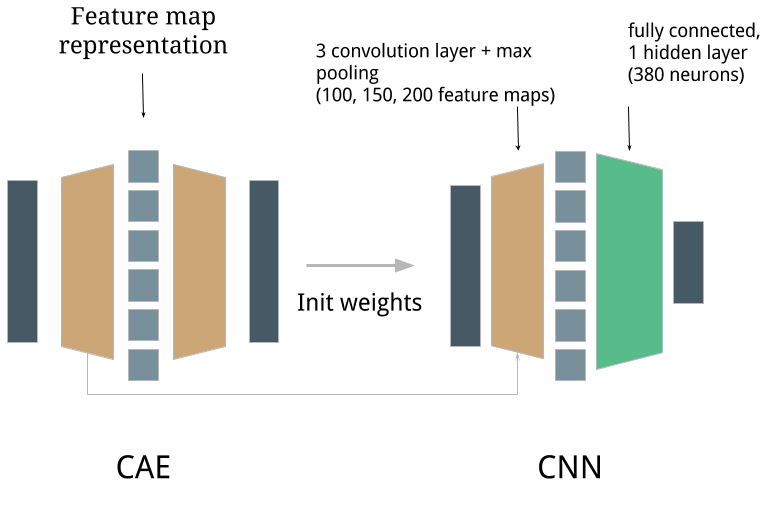
\includegraphics[width=0.6\linewidth]{../graphics/setup.png}
    \caption{Experimental Setup}
    \label{fig:experimental_setup}
  \end{figure}

  In this paper, we evaluate the influence of CNN pre-training using convolutional autoencoders on the network's out-of-sample accuracy. To achieve this, we train, in a first step, a convolutional autoencoder on a chosen dataset and then, in a second step, use its convolution layer weights to initialize the convolution layers of a CNN. After training, we compare the CNN's test set accuracy to a reference network that was trained under the same conditions with randomly initialized convolution weights. 

  A visualization of the weight transfer can be seen on the schematic in figure ~\ref{fig:experimental_setup}. 

  While we restricted the training set size for some of the CNN training experiments, the CAEs were always trained on all available training data since in a lot of settings, additional unlabeled data is easily available while labeled data might be extremely rare and costly.  

  \subsection{Autoencoder}
  \label{sec:methods_autoencoder}

    \paragraph{Architecture}
    The convolutional autoencoder first uses several convolution layers and pooling layers to transform the input to a high dimensional feature map representation and then reconstructs the input using strided transposed convolutions 
    % (TODO: similar to Zeiler / first GAN layers? + citation). 
    In our experiments, we use the autoencoder architecture described \citep{masci2011stacked}. Its encoding part, consisting of 3 times a convolution layer followed by 2x2 non-overlapping max-pooling and a layer of scaled-tanh activations(\ref{par:activation_function}, is described in table \ref{table:encoding_architecture}. All convolutional layer perform a full, non-strided convolution operation and therefore do not change the height/width of the input. 

    \begin{table}[h]

      \centering

      \addvbuffer[10pt]{
        \makebox[0pt]{
          \begin{tabular}{ l|c c c c c c }
            Layer Type    &   input   & convolution     & max-pool  & convolution & max-pool  & convolution \\
            Filter Size   &   none    & 5x5             & 2x2       & 5x5         & 2x2       & 3x3         \\
            Channels      &   1(gray)|3(rgb)   & 100             & 100       & 150         & 150       & 200         \\
            Activation    &   none    & scaled-tanh     & none      & scaled-tanh & none      & scaled-tanh \\
            Size          & $(H,W,C)$ & $(H,W,100)$     & $(\frac{H}{2}, \frac{W}{2}, 100)$ & $(\frac{H}{2}, \frac{W}{2}, 150)$ & $(\frac{H}{4}, \frac{W}{4}, 150)$ & $(\frac{H}{4}, \frac{W}{4}, 200)$
          \end{tabular}
        }
      }
        
      \caption{CAE/CNN: shared encoding layers. Channels refers to the amount of feature maps in the given layer}
      \label{table:encoding_architecture}

    \end{table}

    % $$input \rightarrow conv1 ~(5x5~filter, 100~feature~maps) \rightarrow 2x2 non-overlapping max-pooling \rightarrow activation function \rightarrow  $$

    %In our experiments, the encoding part consisted of:
    % in general: conv layers have (1,1,1,1) strides and we are performing a full convolution (out hei/wid = in hei(wid))
    %input (batchsize, height, width, numchannels) -> conv1 (5x5 filter) (batchsize, height, width, 100) -> activation function (scaled tanh) (b,h,w,100) -> max pooling (2x2, (1,2,2,1) strides) (b, h/2, w/2, 100) -> conv2 (5x5 filter) (b, h/2, w/2, 150) -> activation function (Scaled tanh) (b, h/2, w/2, 150) -> max  pooling (2x2 filter, (1,2,2,1) strides (b, h/4, w/4, 150) -> conv3 (3x3 filter), (b, h/4, w/4, 200) -> activation function (scaled tanh) (b, h/4, w/4, 200) 

    For the reconstruction, we use une strided transpose convolution layer per convolution / max-pool layer in the encoding layers. The weights of the transpose convolutions are the same as learned in the convolution layers and the 2x2 strides invert the downsampling effect of the max-pooling layers.

    \paragraph{Activation Function}
    \label{par:activation_function}
    Out of 3 tested activation functions (sigmoid, scaled tanh and relu), we use the scaled tanh for our main experiments similar to \citep{masci2011stacked}. We will talk about our ReLU experiments in (TODO: add link). With scaled tanh we mean the tanh function rescaled and shifted to the [0,1] output range. This corresponds to the function $$scaledtanh(x) = \frac{1}{2}tanh(x) + \frac{1}{2}$$ which has a generally sigmoidal shape but a stronger gradient around $x = 0$. In our experiments, switching the activation function from sigmoid to scaled tanh seemed to give similarly good results after less training training iterations. 

    \paragraph{Regularization} 
    While autoencoders are typically used for dimensionality reduction, the feature map representation of the convolutional autoencoders we are using is of a much higher dimensionality than the input images. While this feature representation seems well-suited in a CNN, the overcomplete representation becomes problematic in an autoencoder since it gives the autoencoder the possibility to simply learn the identity function. 
    Without any further constraints, a full convolutional layer could easily learn a simple point filter such as $k = \begin{smallmatrix} 0&0&0\\ 0&1&0 \\ 0&0&0 \end{smallmatrix}$ (for grayscale input) that copies the input onto a feature map. While this would later simplify a perfect reconstruction of the input, the CAE does not find any more suitable representation for our data. 
    To prevent this problem, some kind of regularization is needed. 

    Several methods can be found in the literature, most of them involving some kind of sparsity constraint for the representation layer (TODO: cite WTA CAE paper). In \citep{masci2011stacked} the authors use max-pooling as an elegant way to enforce the learning of plausible filters without the need for any further regularization. Since the CNN architecture we are going to use later will contain pooling layers anyways, we stick with this technique and choose not to add any noise to our inputs either since this does not seem not to help the emergence of more natural filters in their experiments. 
    % (TODO: describe what is a natural filter for us). 

    \paragraph{Training} While the authors of \citep{masci2011stacked} use a layer-wise training for convolutional autoencoders, we achieve good results by training the whole auto-encoder at once. 
    % (TODO: maybe this made it more difficult / longer to train?).
    For the \emph{MNIST} and \emph{CIFAR-10} datasets, the autoencoders are trained with simple gradient descent using as learning rate of $lr = 0.5$, for the CKPLUS dataset, we use the adagrad optimizer with the same initial learning rate $lr$.\footnote{CAE convolution filters initialized using a truncated normal distribution ($\mu = 0.001$, $\sigma = 0.05$), all bias values initialized with the constant $0.001$}

  \subsection{CNN Pre-Training}

    \paragraph{CNN architecture} The CNN uses the same architecture as the CAE encoding for its convolution layers (feature extraction) and then uses two fully-connected layers (sizes 384 and 10) for decision making, the first having a scaled tanh activation, the second followed by a softmax layer for probabilistic output.

    \paragraph{CNN Initialization and Training}

    % INITIALIZATION
    The convolutional layer weights (filters) and biases of the pre-trained networks were initialized with the values obtained from the convolutional autoencoders. The reference CNN's convolution weights were initialized with mean $\mu = 0 $ and standard deviation $\sigma = 0.2$, the biases with the constant value $b =  0.0001$.

    The fully-connected layers were initialized randomly for all networks. \footnote{CNN fully-connected layer weights initialized with a truncated normal distribution ($\mu = 0$, $\sigma = 0.001$), biases with the constant value $0.0001$.}
    This means that for all experiments, some parts of the networks are randomly initialized, all weights for the reference networks and the fully-connected weights for the pre-trained networks. 

    % TRAINING 
    % (TODO: optimizer, step size, convergence criterion, amount of epochs per dataset)
    For each datset, we split the available training data into training and evaluation set and use the evaluation set to track the training progress and adjust hyperparameters. We keep track of both cross-entropy error and accuracy on the evaluation set and stop training when these values converge. Afterwards, we evaluate the networks accuracy once on the held-out test set and use the obtained value as a result. We let every experimental setup run 10 times, average the results and conduct a t-test for significante. The test set stays the same over all runs. 
 
    For the larger datasets \emph{MNIST} and \emph{CIFAR-10}, we conduct several experiments restricting the amount of available training data inspired by \citep{masci2011stacked}. The autoencoder used for pre-training is always trained on the whole dataset. 

    Since we are working with small amounts of training images for complex datasets, we are aware that problems with overfitting might arise. In order to prevent these effects, we use dropout regularization in the dense layers~footnote{using a dropout rate of 0.5 during training time}, monitor the training progress with a seperate validation set and measure the generalization performance on a held-out test set. 

    %\begin{itemize}
      %\item Network Architectures
      %\item Weight Transfer
      %\item weight initialization (all layers)
      %\item CNN Training
      %\item Test Methodology (Train + Validation + Test Sets)
      %\item 1k/10k/full splits but always full dataset for CAE
    %\end{itemize}

  %\subsection{Evaluation}
  %  For each dataset and training size, we train k pre-trained CNNs and k randomly initialized reference CNNs.
  %  (TODO: add better description + significance test)

  \subsection{Extended Cohn-Kanade Dataset}

      \begin{figure}%[h]
        \centering
        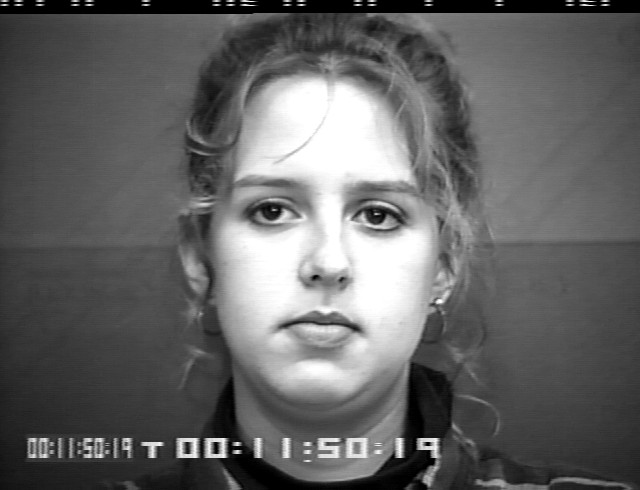
\includegraphics[width=0.15\linewidth]{../graphics/ckplus_frames/S052_001_00000001.png}
        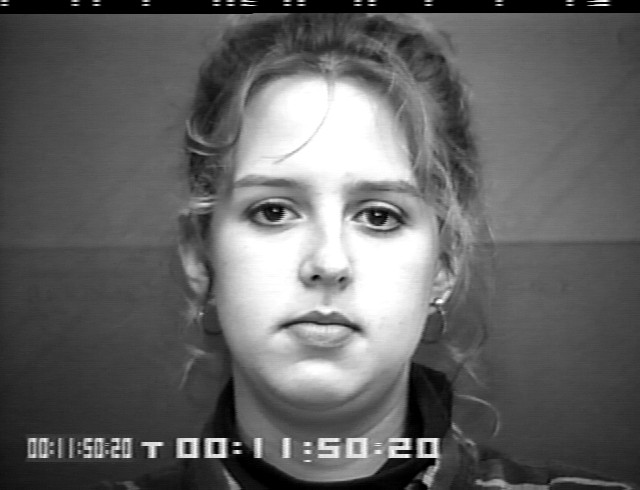
\includegraphics[width=0.15\linewidth]{../graphics/ckplus_frames/S052_001_00000002.png}
        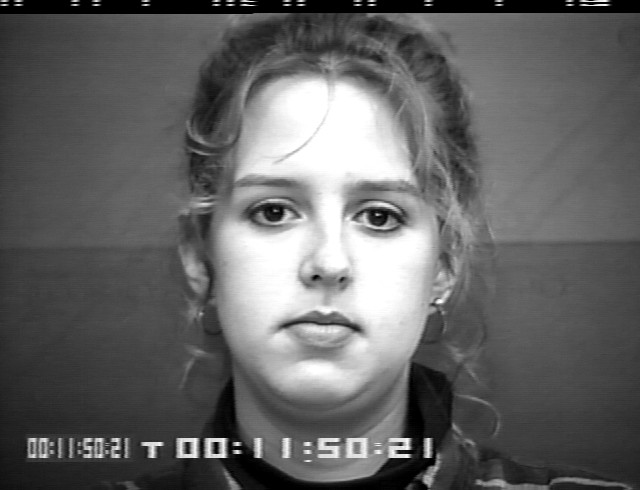
\includegraphics[width=0.15\linewidth]{../graphics/ckplus_frames/S052_001_00000003.png}
        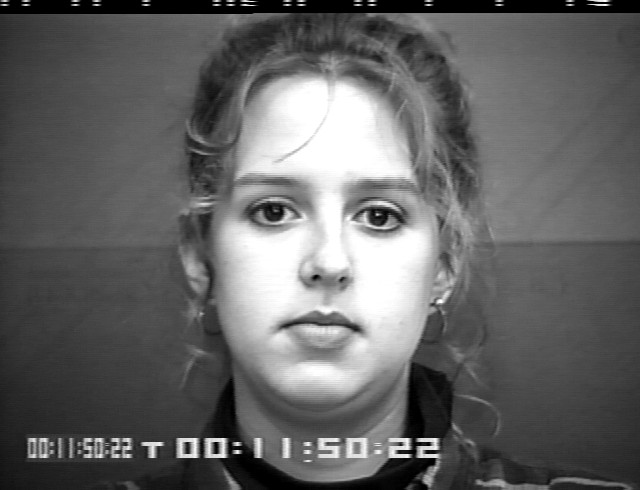
\includegraphics[width=0.15\linewidth]{../graphics/ckplus_frames/S052_001_00000004.png}
        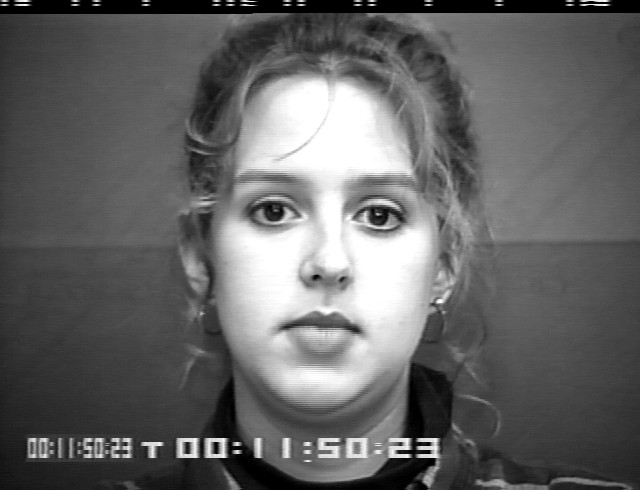
\includegraphics[width=0.15\linewidth]{../graphics/ckplus_frames/S052_001_00000005.png}

        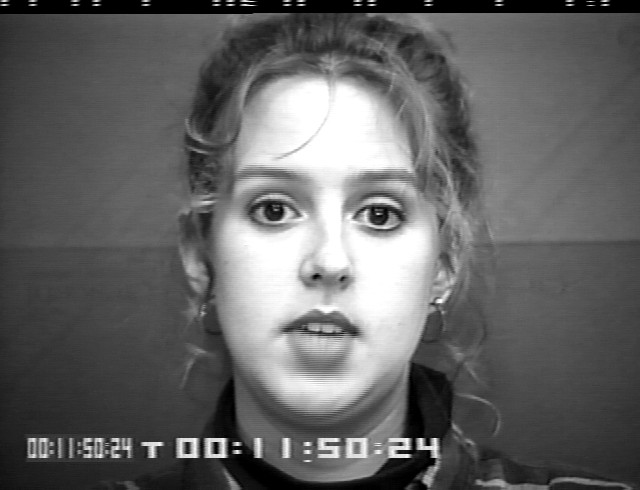
\includegraphics[width=0.15\linewidth]{../graphics/ckplus_frames/S052_001_00000006.png}
        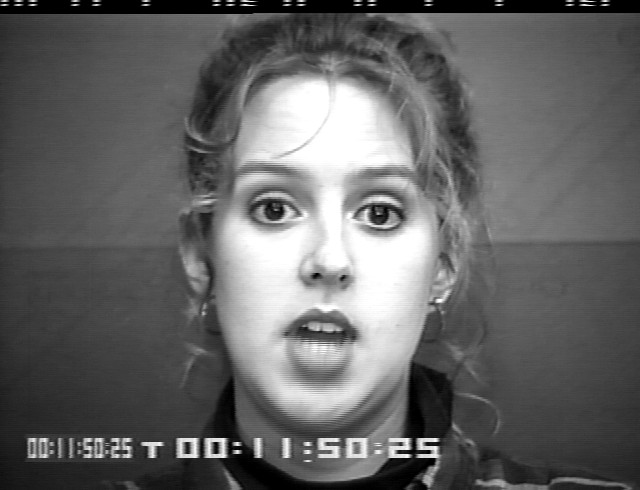
\includegraphics[width=0.15\linewidth]{../graphics/ckplus_frames/S052_001_00000007.png}
        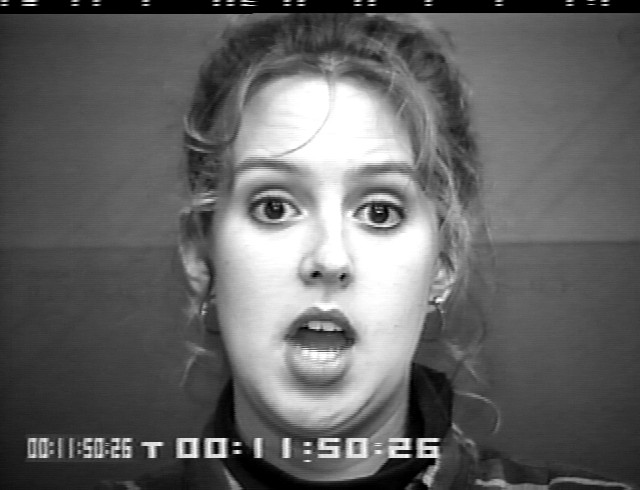
\includegraphics[width=0.15\linewidth]{../graphics/ckplus_frames/S052_001_00000008.png}
        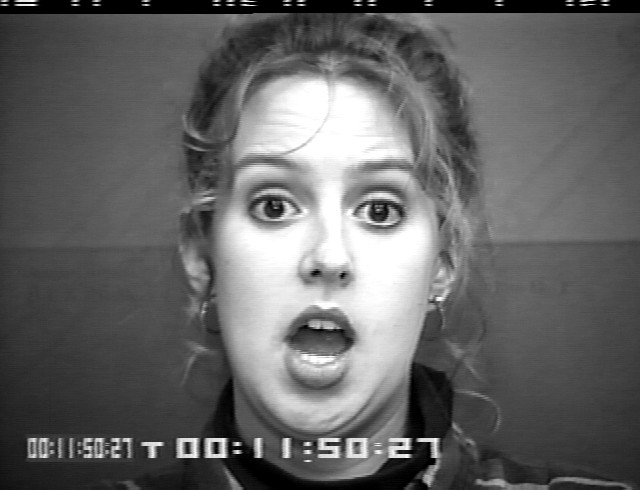
\includegraphics[width=0.15\linewidth]{../graphics/ckplus_frames/S052_001_00000009.png}
        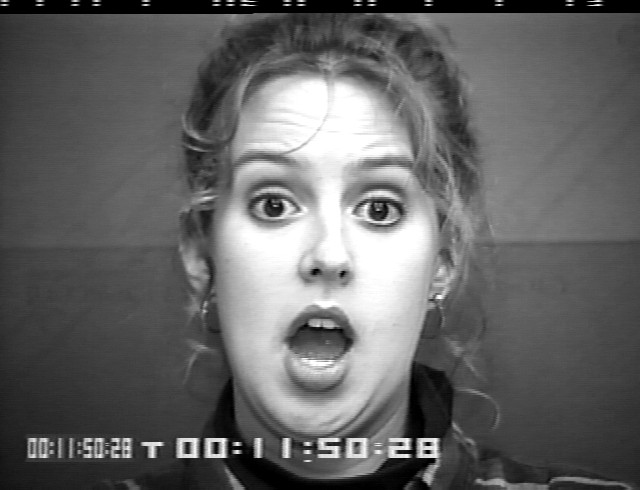
\includegraphics[width=0.15\linewidth]{../graphics/ckplus_frames/S052_001_00000010.png}

        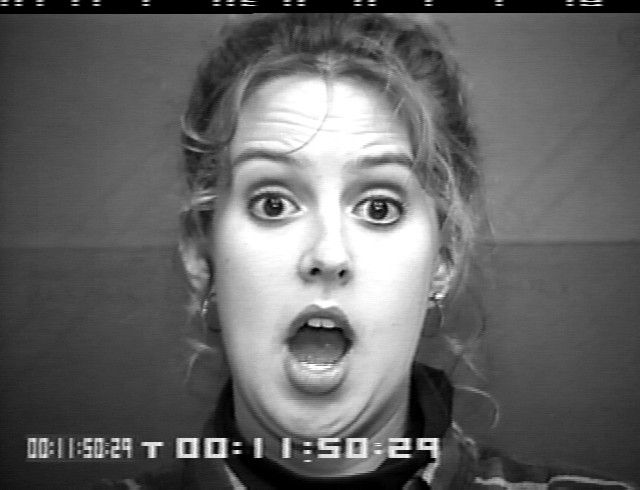
\includegraphics[width=0.15\linewidth]{../graphics/ckplus_frames/S052_001_00000011.png}
        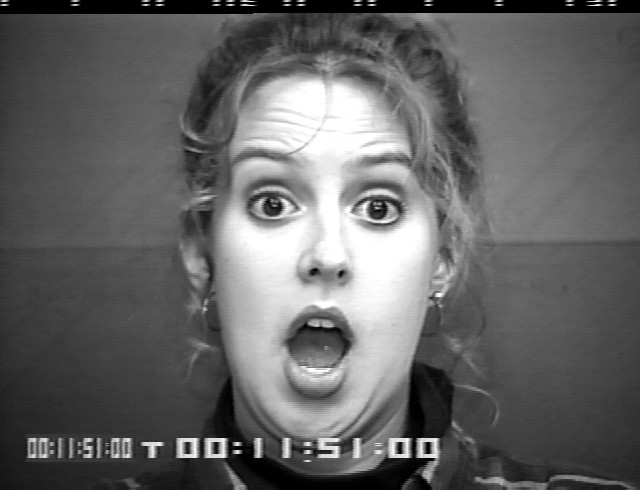
\includegraphics[width=0.15\linewidth]{../graphics/ckplus_frames/S052_001_00000012.png}
        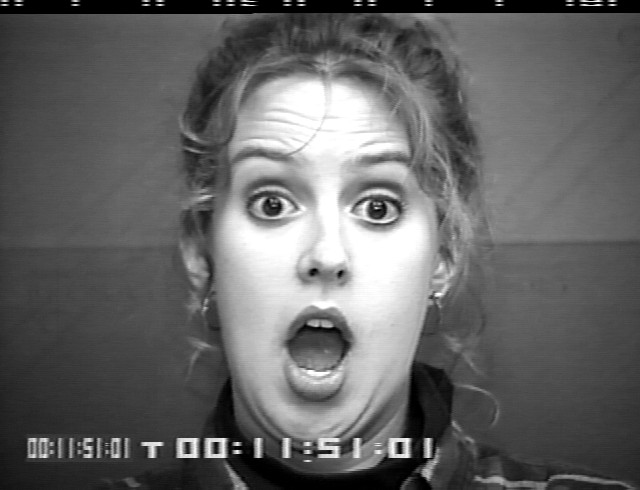
\includegraphics[width=0.15\linewidth]{../graphics/ckplus_frames/S052_001_00000013.png}
        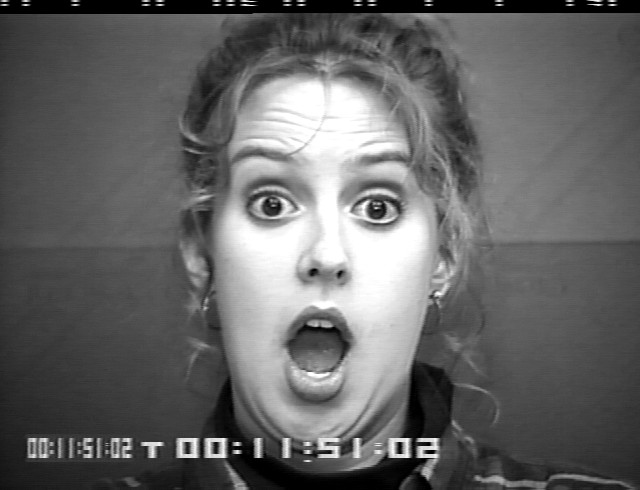
\includegraphics[width=0.15\linewidth]{../graphics/ckplus_frames/S052_001_00000014.png}
        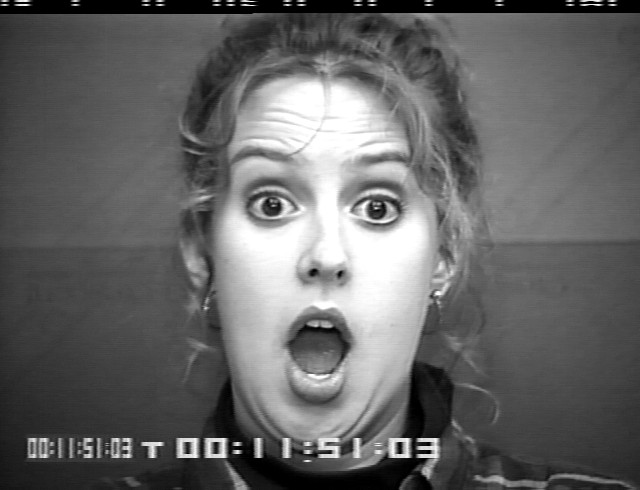
\includegraphics[width=0.15\linewidth]{../graphics/ckplus_frames/S052_001_00000015.png}

        \caption{CK+ frames from neutral face to emotional face ({\textcopyright}Jeffrey Cohn)}
        \label{fig:ckplus_frames}
      \end{figure}

      Alltogether the Extended Cohn-Kanade (CK+) dataset \citep{kanade2000comprehensive,lucey2010extended} has 123 subjects and 593 emotion sequences, which are 10-60 frames of short video sequences, from a neutral face to the target emotion, as can be seen in figure \ref{fig:ckplus_frames}
      CK+ is the most interesting dataset in our project, as unlike the other two datasets, no pre-training experiments have been done on CK+, as far as we know.

      As the CK+ dataset is not readily prepared for running those kinds of experiments, we have to put some work into this ourselves.
      We decided to not take the full images, but use the provided facial landmarks, to put the faces into a bounding box and scale them down by factor 5 to a size of 68x65 pixels.
      In order to train the autoencoder we use all of the frames as unlabelled input, for the CNN we use the last three frames of all sequences, labelled with the target emotion.
      We split the dataset into training, validation and test set by subject, so that we end up with 696 training, 87 validation and 198 test images for the CNN.
      Before training we randomly shuffle the images and used the same split for all runs.

      Another specialty for the CK+ dataset is, that when we use all frames for the CAE, this includes frames which are neutral or even ambiguous.
      As this possibly broadens the available information for learning the autoencoder, and is also useful for practical use, we could possibly use a lot of unlabelled images for pre-training.
      In this case the pretraining makes especially sense, because we can learn features, we could not learn when training only a CNN with labelled images.

  \subsection{Statistical Significance}
      In order to validate possible resulting accuracy differences, we also want to check their significance.
      Therefore we run a standard t-test to measure if the accuracies from the randomly initialized CNN are significantly different from the pre-trained one.
      This way we calculated the probability (p-value) that the improvements could occur, when the pretrained network was not better than the randomly initialized one (Null-hypothesis).


\section{Experimental Results}
  % Results and challenges while performing experiments
  % Training process
  % FOCUS: CK+ Processing & describe experiments exactly
  We conducted experiments on the three introduced datasets (MNIST, CIFAR-10 and CK+) datasets, which vary in their image size, number of images and colour information.
  
  \subsection{Autoencoder Reconstruction}
    % For the autoencoder training we took each of the three datasets' images, reshaped them into a vector and used these values as input and target output for a convolutional autoencoder. The architecture for the autoencoder was chosen in a way, so that the CNN would give best results.

    % For the loss function we decided to use the mean-squared error, as cross-entropy did not give us good results. % Maybe add explanation? Only if enough time
    When training a utilizable convolutional autoencoder (CAE), the most obvious goal is to get good reconstructions of the input images.
    Even though this does not always necessarily mean that we learned a good representation, it was still our main optimization criteria here.
    In the next section we will then check, if we actually learned a useful representation by applying it to a classification network.

    After 300k training iterations on a dataset, the CAE reconstructs the input images sucesfully, examples can be seen in figure \ref{fig:mnist_reconstructions}, \ref{fig:cifar_reconstructions} and \ref{fig:ckplus_reconstructions}. While the reconstructions for the simple \emph{MNIST} dataset are almost perfect, the reconstructed images on the \emph{Cifar} and \emph{CK+} datasets seem like blurred versions of the input images, however the main features are still visible and on \emph{CK+}, the emotions are clearly differentiable. All autoencoders have the same architecture as described in \ref{sec:methods_autoencoder} and use the scaled tanh as activation function. The learned first layer filters show a similar structure to the ones shown in \citep{masci2011stacked}\footnote{Example filters can be seen on \emph{Github} \url{https://github.com/gangchill/nip-convnet/tree/master/experiments/paper_reference_experiments/paper_reference_cae/cifar}}. 

    \begin{figure}% [ht]
      \centering

      \begin{subfigure}{0.45\linewidth}

      
\includegraphics[width=0.3\linewidth]{../graphics/reconstructions/mnist/input_00.png}
      
\includegraphics[width=0.3\linewidth]{../graphics/reconstructions/mnist/input_01.png}
      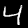
\includegraphics[width=0.3\linewidth]{../graphics/reconstructions/mnist/input_02.png}

      
\includegraphics[width=0.3\linewidth]{../graphics/reconstructions/mnist/reconstruction_00.png}
      
\includegraphics[width=0.3\linewidth]{../graphics/reconstructions/mnist/reconstruction_01.png}
      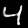
\includegraphics[width=0.3\linewidth]{../graphics/reconstructions/mnist/reconstruction_02.png}

      \caption{\emph{MNIST} example images (top) and CAE reconstructions (bottom)}
      \label{fig:mnist_reconstructions}

      \end{subfigure}
      \begin{subfigure}{0.45\linewidth}
        
      %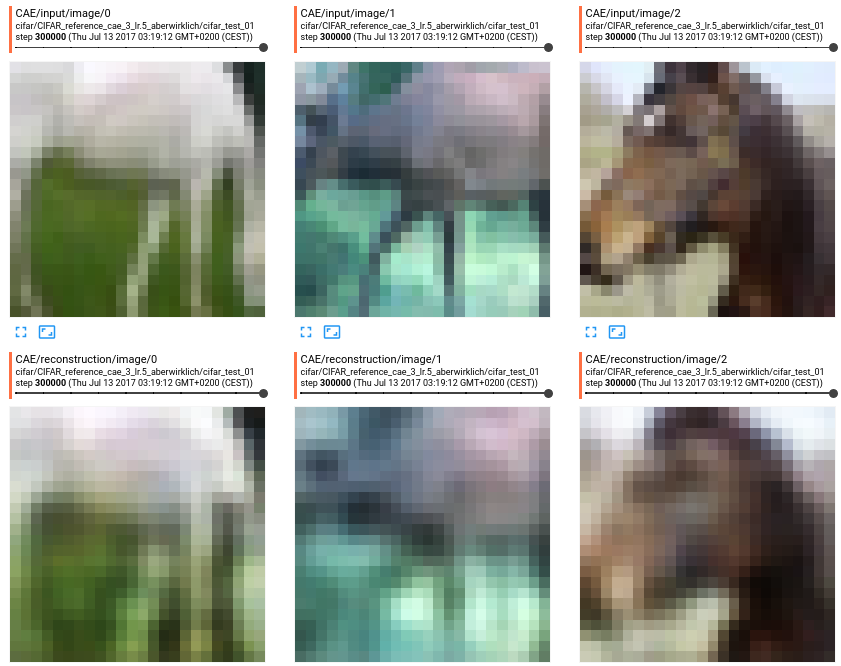
\includegraphics[width=0.8\linewidth]{../graphics/cifar_reconstructions.png}
      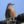
\includegraphics[width=0.3\linewidth]{../graphics/reconstructions/cifar/input_00.png}
      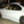
\includegraphics[width=0.3\linewidth]{../graphics/reconstructions/cifar/input_01.png}
      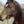
\includegraphics[width=0.3\linewidth]{../graphics/reconstructions/cifar/input_02.png}

      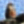
\includegraphics[width=0.3\linewidth]{../graphics/reconstructions/cifar/reconstruction_00.png}
      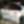
\includegraphics[width=0.3\linewidth]{../graphics/reconstructions/cifar/reconstruction_01.png}
      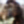
\includegraphics[width=0.3\linewidth]{../graphics/reconstructions/cifar/reconstruction_02.png}

      \caption{\emph{CIFAR-10} example images(top) and CAE reconstructions(bottom)}
      \label{fig:cifar_reconstructions}

      \end{subfigure}
      

    \end{figure}

    \begin{figure}% [h]
      \centering
      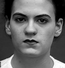
\includegraphics[width=0.2\linewidth]{../graphics/reconstructions/ckplus/input_00.png}
      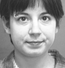
\includegraphics[width=0.2\linewidth]{../graphics/reconstructions/ckplus/input_01.png}
      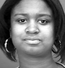
\includegraphics[width=0.2\linewidth]{../graphics/reconstructions/ckplus/input_02.png}

      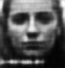
\includegraphics[width=0.2\linewidth]{../graphics/reconstructions/ckplus/reconstruction_00.png}
      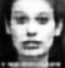
\includegraphics[width=0.2\linewidth]{../graphics/reconstructions/ckplus/reconstruction_01.png}
      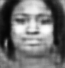
\includegraphics[width=0.2\linewidth]{../graphics/reconstructions/ckplus/reconstruction_02.png}

      %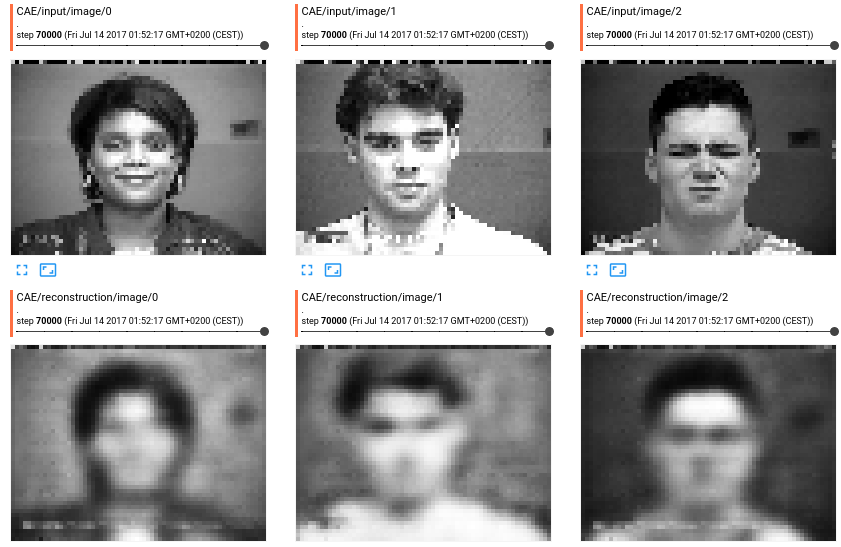
\includegraphics[width=0.8\linewidth]{../graphics/ckplus_reconstructions_better.png}
      \caption{CK+ input image (top) and reconstruction (bottom) ({\textcopyright}Jeffrey Cohn)}
      \label{fig:ckplus_reconstructions}
    \end{figure}

    \subsubsection{Rectified Linear Units}
      When switching to a ReLu activation function \citep{nair2010rectified} for the CAE, the reconstructions become almost identical to the input image, but the learned first layer filters seem rather random compared to the ones obtained in previous experiments. Since first pre-training results do not show a significant change between pre-trained and randomly initialized ReLU networks, we do not examine this setting more in detail. Example reconstructions and a random selection of first layer filters are shown in figure \ref{fig:relu_cae}.

      \begin{figure}[b]

      \centering

				\begin{subfigure}{0.4\linewidth}

					\centering
					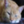
\includegraphics[width=0.4\linewidth]{../graphics/reconstructions/cifar/relu/input_00_relu.png}
					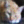
\includegraphics[width=0.4\linewidth]{../graphics/reconstructions/cifar/relu/reconstruction_00_relu.png}
					%\caption{(CAE:) Reconstruction example using ReLU activation + smaller network size}

				\end{subfigure}
				\begin{subfigure}{0.4\linewidth}

					\centering
					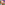
\includegraphics[width=0.1\linewidth]{../graphics/reconstructions/cifar/relu/relu_filter_00.png} \hspace{0.05\linewidth}
					
\includegraphics[width=0.1\linewidth]{../graphics/reconstructions/cifar/relu/relu_filter_01.png} \hspace{0.05\linewidth}
					
\includegraphics[width=0.1\linewidth]{../graphics/reconstructions/cifar/relu/relu_filter_02.png} \\
					\vspace{0.05\linewidth}
					
\includegraphics[width=0.1\linewidth]{../graphics/reconstructions/cifar/relu/relu_filter_03.png} \hspace{0.05\linewidth}
					
\includegraphics[width=0.1\linewidth]{../graphics/reconstructions/cifar/relu/relu_filter_04.png} \hspace{0.05\linewidth}
					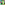
\includegraphics[width=0.1\linewidth]{../graphics/reconstructions/cifar/relu/relu_filter_05.png} \\
					\vspace{0.05\linewidth}
					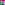
\includegraphics[width=0.1\linewidth]{../graphics/reconstructions/cifar/relu/relu_filter_06.png} \hspace{0.05\linewidth}
					
\includegraphics[width=0.1\linewidth]{../graphics/reconstructions/cifar/relu/relu_filter_07.png} \hspace{0.05\linewidth}
					
\includegraphics[width=0.1\linewidth]{../graphics/reconstructions/cifar/relu/relu_filter_08.png} 

					%\caption{(CAE:) Structureless first layer filters learned by ReLU autoencoder}

				\end{subfigure}

			\caption{\textbf{ReLU CAE} example input + reconstruction (left), selection of first layer filters (right) }
			\label{fig:relu_cae}

    \end{figure}

  \subsection{Pretraining and Classification}
%    The general idea of pretraining a classification neural network, is to transfer the encoding weights of the CAE to the CNN. So we took the convolutional filter weights, which we generated during the autoencoder training, and used them as initial values for the convolutional layers for the classification network.

 %   As the MNIST and CIFAR-10 datasets consist of a lot more images than CK+, we decided to follow the approach of the paper and take a 1k and 10k subset for these two. So while we still took all training images for building a decent autoencoder, the CNN could only use some of the images. This is especially interesting to check the hypothesis, that pre-training makes more sense, when you have less training images.

  %  To validate our pretraining experiments, in each run we set up a CNN with randomly initialized filters and a CNN which uses the filters trained by the CAE. Both networks have randomly initialized weights for their dense layers.
    As described above to validate the pre-training advantage we trained randomly initialized netwforks and networks which contain the pre-trained feature maps.

    We let all networks train till we observed conversion, and then used this empircally obtained number of iterations for all following trainings.
    The length of training was at least 30 epochs for all datasets, so 5k iterations for the 1k datasets, 10k iterations for the 10k datasets and 20k iterations for the full datasets of MNIST and CIFAR-10.
    CK+ has been trained for 2k iterations, this corresponds to more than 350 epochs.
    During this we checked for overfitting, but did not notice a big trend for it.
    So apparently our regularization mostly works fine.

    After the final training we measure the classification accuracy on the separate testset for both the random-initialized and the pre-trained CNN, so that we can measure generalization and compare the results.
    
    % experimental results:
    As can be seen in figures \ref{fig:mnist_cifar_plot} and \ref{fig:ckplus_plot}, accuracy values for the pre-trained networks are higher for almost all datasets and configurations. The only exception is the \emph{CIFAR-10} dataset with a training set of 1000 images. When looking at results of the t-test in table \ref{table:significance}, there is a significant difference for almost all dataset configurations, the only outlier being again \emph{CIFAR} 1k. 
    
    %Cifar-10 overfitting?
    Pre-training consistently outperforms random initialization on almost all dataset configurations. Since \emph{CIFAR-10} with its natural images seems the most complex classification task, we assume that in this scenario overfitting might be more of a problem. We suppose that with additional regularization, pre-training could as well be benificial in this context. 

    \begin{figure}
      \centering

      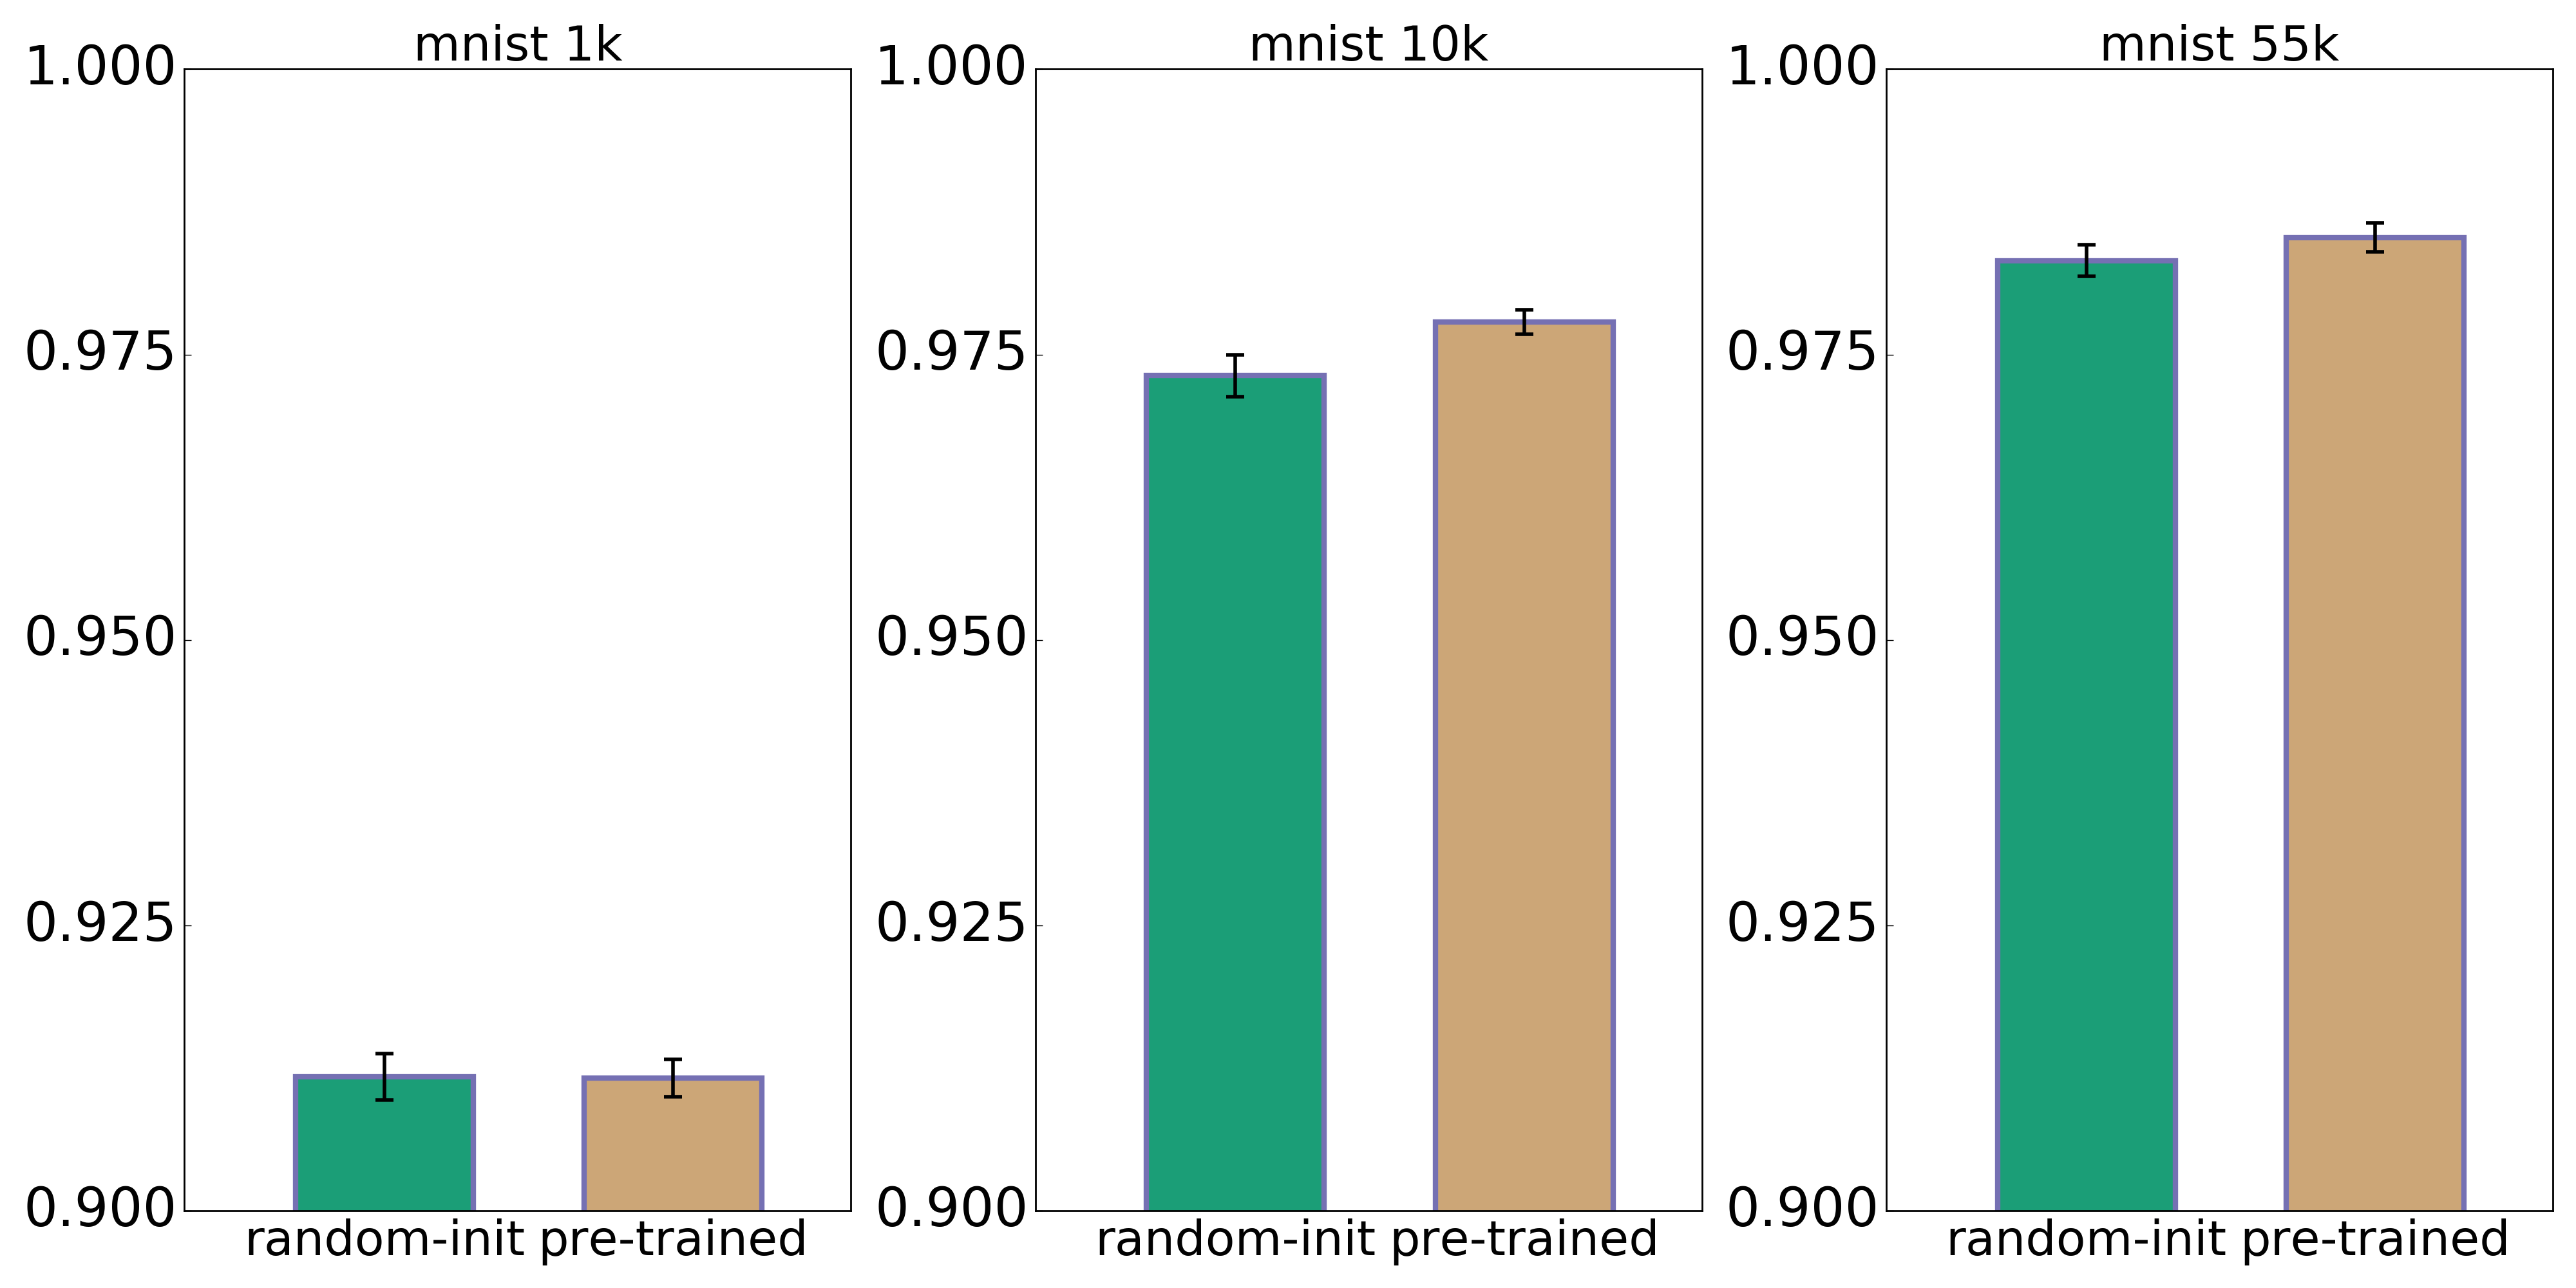
\includegraphics[width=.8\linewidth]{../box_plots/boxplots_mnist.png}

      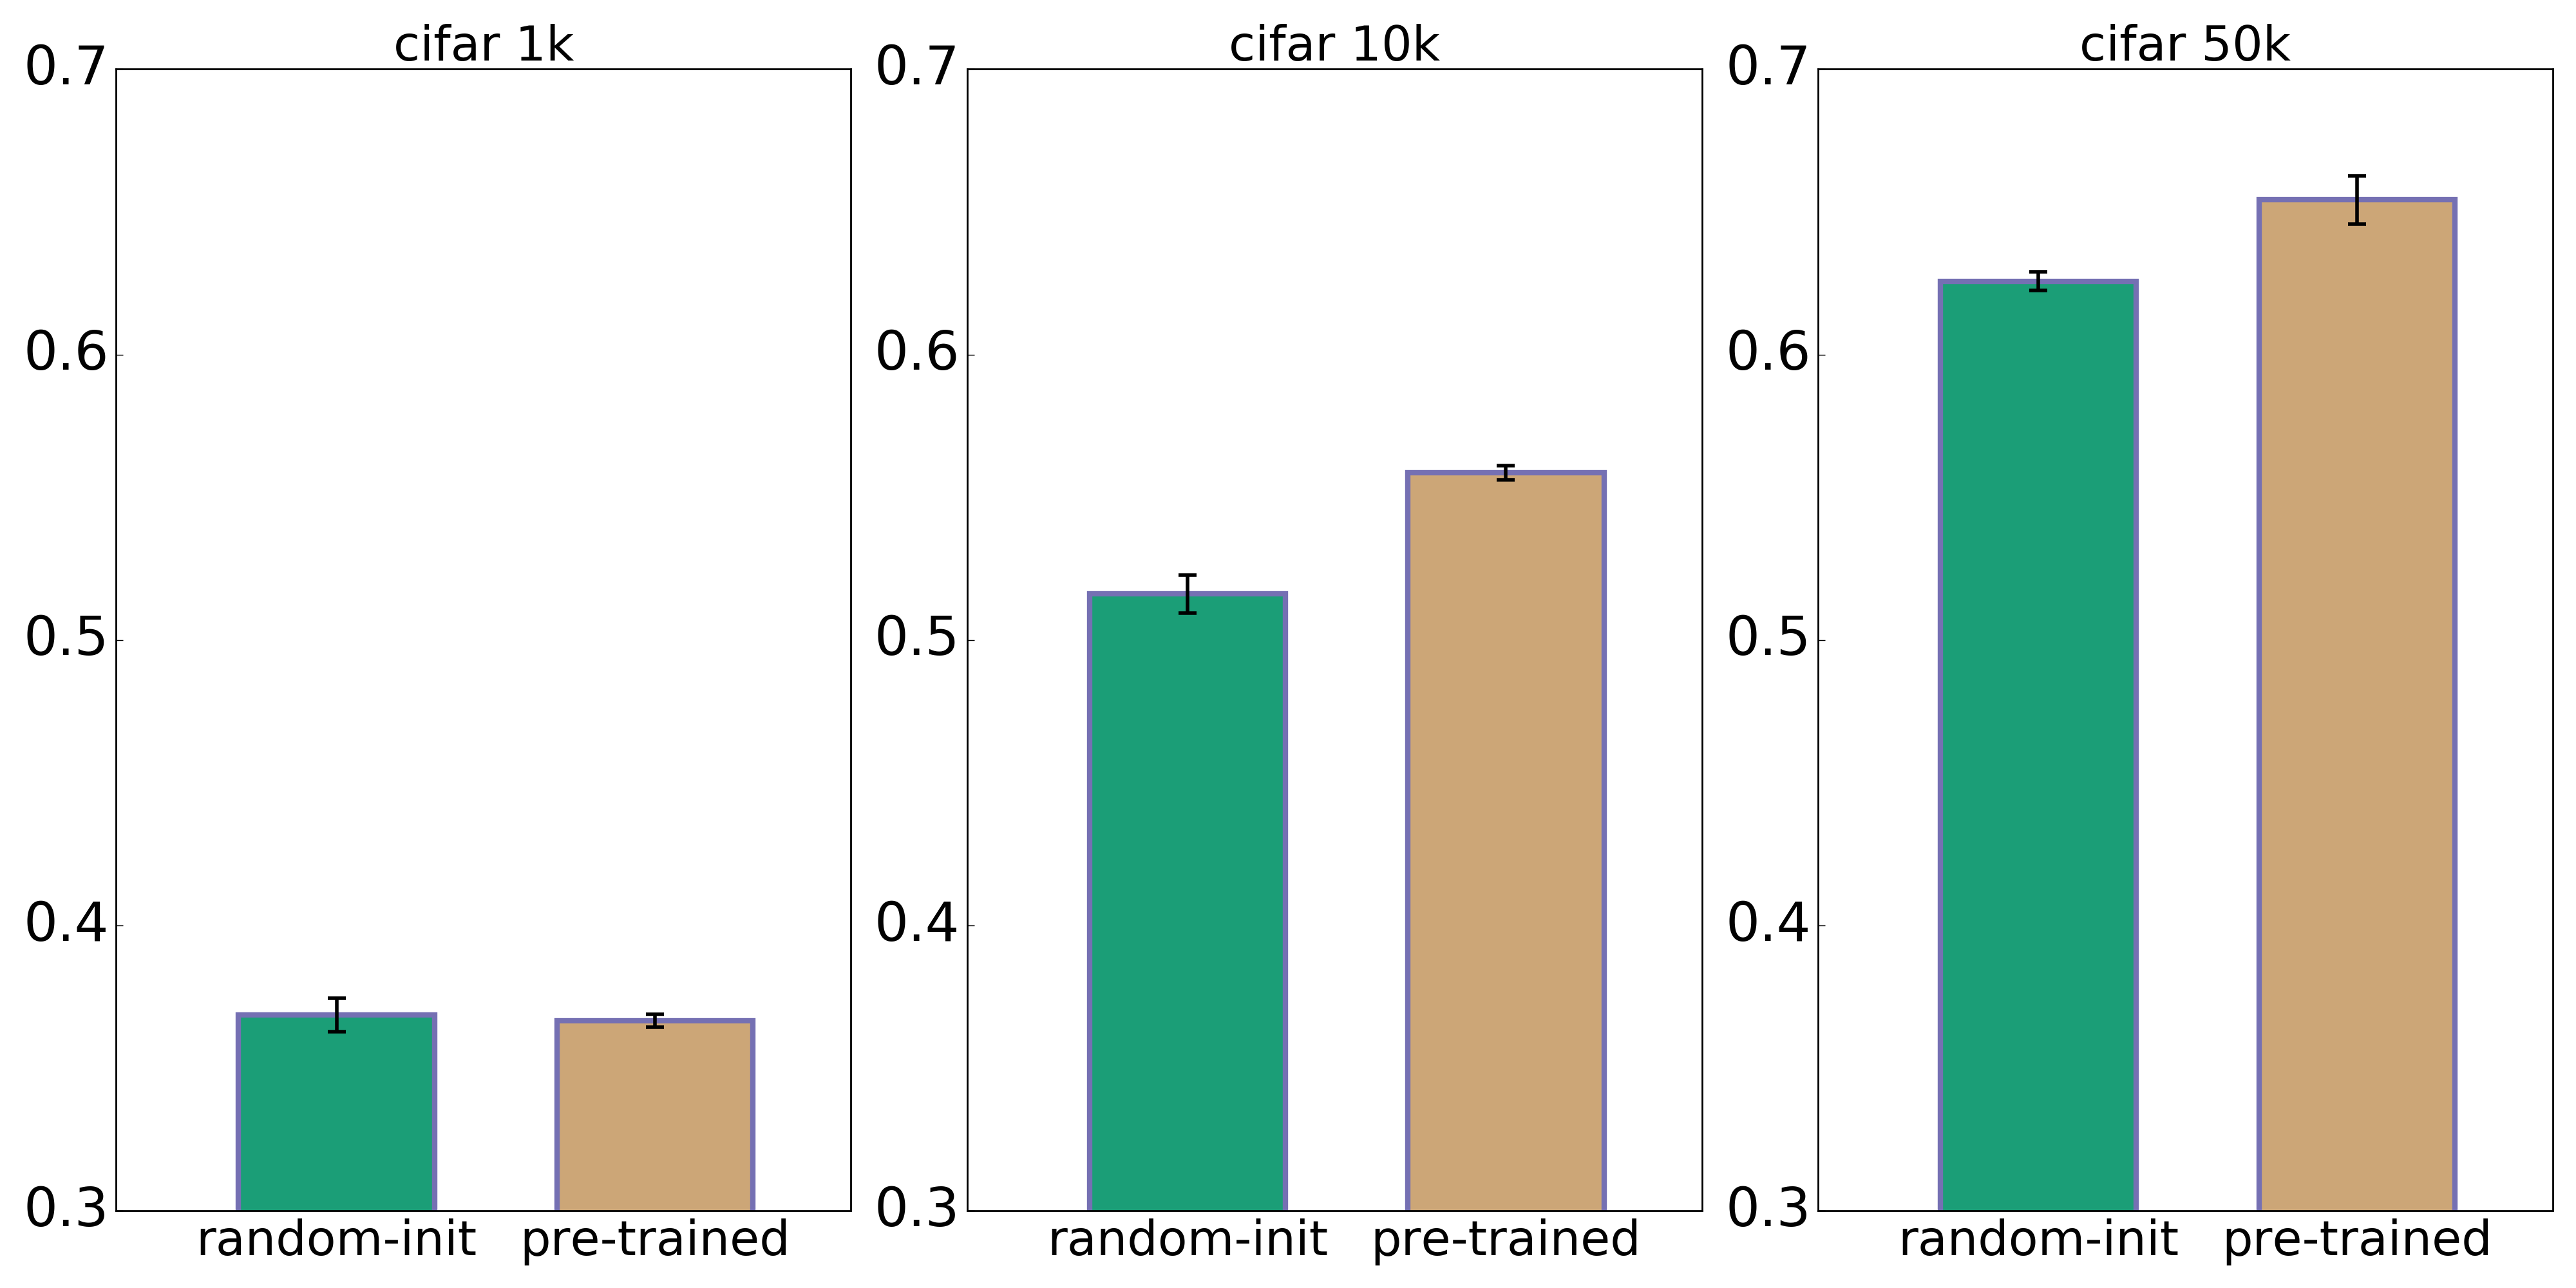
\includegraphics[width=.8\linewidth]{../box_plots/boxplots_cifar.png}

      \caption{Pre-Training Results \emph{MNIST}(top) and \emph{CIIFAR-10}(bottom): Test set accuracy after training on different subsets of the training data.}
      \label{fig:mnist_cifar_plot}
    \end{figure}


    \begin{figure}
      \centering
      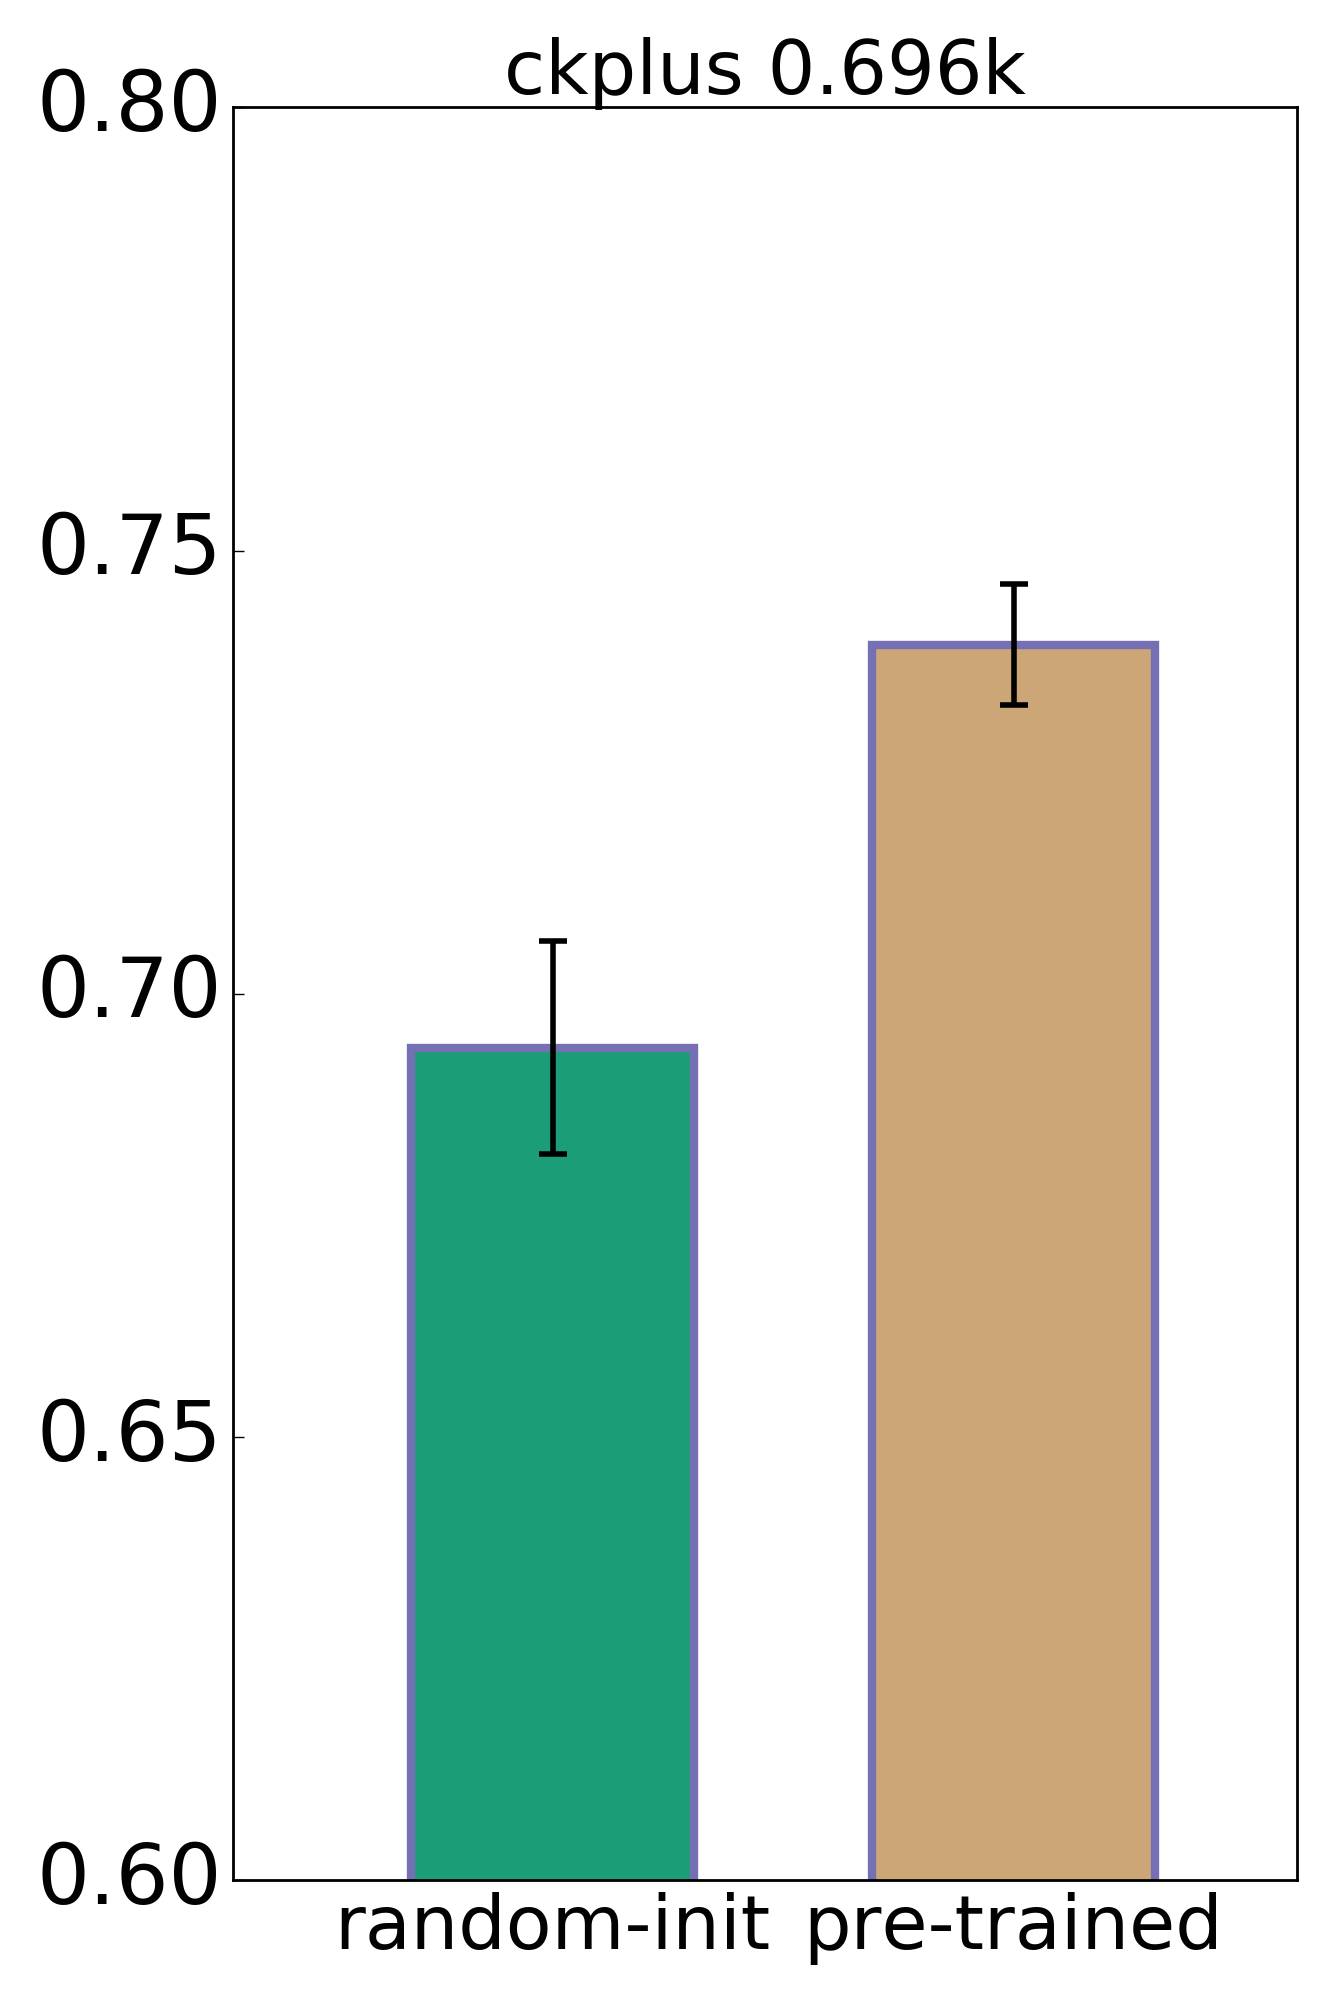
\includegraphics[width=0.33\linewidth]{../box_plots/boxplots_ckplus.png}
      \caption{\emph{CK+}: test set accuracy comparison for 696 training images (stddev in black)}
      \label{fig:ckplus_plot}
    \end{figure}

    In addition to the significant improvement in out-of-sample accuracy, we also observe a striking difference between the filters after convergence depending on the network initialization. The pre-trained networks first-layer filters seem to preserve a lot of the structure learned in the autoencoder, a sign that the learned representation seems to be well suited for the classification task. While the randomly-initialized filters change more during training, their final appearence never shows as clearly interpretable low-level structures as can be seen in an example on the emph{CIFAR-10} dataset in figure~\ref{fig:cifar_filters}.  

      \begin{figure}
          \centering

            \begin{subfigure}{.4\linewidth}
              \centering
              \includegraphics[width=0.1\linewidth]{../graphics/cifar_filters/pre_trained_01.png} 
              \includegraphics[width=0.1\linewidth]{../graphics/cifar_filters/pre_trained_02.png} %\hspace{0.05\linewidth}
              \includegraphics[width=0.1\linewidth]{../graphics/cifar_filters/pre_trained_03.png}
              \includegraphics[width=0.1\linewidth]{../graphics/cifar_filters/pre_trained_04.png} %\hspace{0.05\linewidth}
              \includegraphics[width=0.1\linewidth]{../graphics/cifar_filters/pre_trained_05.png} %\hspace{0.05\linewidth}
              \includegraphics[width=0.1\linewidth]{../graphics/cifar_filters/pre_trained_06.png} \\
              \includegraphics[width=0.1\linewidth]{../graphics/cifar_filters/pre_trained_07.png} %\hspace{0.05\linewidth}
              \includegraphics[width=0.1\linewidth]{../graphics/cifar_filters/pre_trained_08.png} %\hspace{0.05\linewidth}
              \includegraphics[width=0.1\linewidth]{../graphics/cifar_filters/pre_trained_09.png}
              \includegraphics[width=0.1\linewidth]{../graphics/cifar_filters/pre_trained_10.png} 
              \includegraphics[width=0.1\linewidth]{../graphics/cifar_filters/pre_trained_11.png} %\hspace{0.05\linewidth}
              \includegraphics[width=0.1\linewidth]{../graphics/cifar_filters/pre_trained_12.png} \\
              \includegraphics[width=0.1\linewidth]{../graphics/cifar_filters/pre_trained_13.png} %\hspace{0.05\linewidth}
              \includegraphics[width=0.1\linewidth]{../graphics/cifar_filters/pre_trained_14.png} %\hspace{0.05\linewidth}
              \includegraphics[width=0.1\linewidth]{../graphics/cifar_filters/pre_trained_15.png}
              \includegraphics[width=0.1\linewidth]{../graphics/cifar_filters/pre_trained_16.png} %\hspace{0.05\linewidth}
              \includegraphics[width=0.1\linewidth]{../graphics/cifar_filters/pre_trained_17.png} %\hspace{0.05\linewidth}
              \includegraphics[width=0.1\linewidth]{../graphics/cifar_filters/pre_trained_18.png}
              %\caption{\emph{CIFAR-10}(CNN): random first layer filters, pre-trained}
            \end{subfigure}
            \begin{subfigure}{.4\linewidth}
              \centering
              \includegraphics[width=0.1\linewidth]{../graphics/cifar_filters/random_01.png} 
              \includegraphics[width=0.1\linewidth]{../graphics/cifar_filters/random_02.png} %\hspace{0.05\linewidth}
              \includegraphics[width=0.1\linewidth]{../graphics/cifar_filters/random_03.png}
              \includegraphics[width=0.1\linewidth]{../graphics/cifar_filters/random_04.png} %\hspace{0.05\linewidth}
              \includegraphics[width=0.1\linewidth]{../graphics/cifar_filters/random_05.png} %\hspace{0.05\linewidth}
              \includegraphics[width=0.1\linewidth]{../graphics/cifar_filters/random_06.png} \\
              \includegraphics[width=0.1\linewidth]{../graphics/cifar_filters/random_07.png} %\hspace{0.05\linewidth}
              \includegraphics[width=0.1\linewidth]{../graphics/cifar_filters/random_08.png} %\hspace{0.05\linewidth}
              \includegraphics[width=0.1\linewidth]{../graphics/cifar_filters/random_09.png}
              \includegraphics[width=0.1\linewidth]{../graphics/cifar_filters/random_10.png} 
              \includegraphics[width=0.1\linewidth]{../graphics/cifar_filters/random_11.png} %\hspace{0.05\linewidth}
              \includegraphics[width=0.1\linewidth]{../graphics/cifar_filters/random_12.png} \\
              \includegraphics[width=0.1\linewidth]{../graphics/cifar_filters/random_13.png} %\hspace{0.05\linewidth}
              \includegraphics[width=0.1\linewidth]{../graphics/cifar_filters/random_14.png} %\hspace{0.05\linewidth}
              \includegraphics[width=0.1\linewidth]{../graphics/cifar_filters/random_15.png}
              \includegraphics[width=0.1\linewidth]{../graphics/cifar_filters/random_16.png} %\hspace{0.05\linewidth}
              \includegraphics[width=0.1\linewidth]{../graphics/cifar_filters/random_17.png} %\hspace{0.05\linewidth}
              \includegraphics[width=0.1\linewidth]{../graphics/cifar_filters/random_18.png}
              %\caption{\emph{CIFAR-10}(CNN): random first layer filters, random-init}
            \end{subfigure}

          \caption{\textbf{\emph{CIFAR-10} CNN} selection of first layer filters. pre-trained (left), random-init (right)}
          \label{fig:cifar_filters}

      \end{figure}


    \begin{table}
      \caption{Statistical Significance of Pretraining Improvements}
      \label{table:significance}
      \centering
      \begin{tabular}{llcl}
        \toprule
        %\multicolumn{2}{c}{Part}                   \\
        %\cmidrule{1-2}
        Dataset     & Size    & Average Accuracy Improvement & Significance (p-value) \\
        \midrule
        MNIST & 1k    & + 0.37 \%  & < 5e-4 \\
              & 10k   & + 0.39 \%  & < 5e-4 \\
              & 50k   & + 0.32 \%  & < 1e-2 \\
        \midrule
        CIFAR-10  & 1k    & - 0.20 \% & > 0.35\\
                  & 10k   & + 4.25 \% & < 1e-9\\
                  & 50k   & + 2.85 \% & < 1e-6\\
        \midrule
        CK+     & 1k & + 4.5 \%      & < 1e-7 \\
        \bottomrule
      \end{tabular}
    \end{table}

    \subsubsection{Interpretation}
      For both MNIST and CIFAR-10 it can be observed, that the accuracy on a pre-trained CNN is higher than with a randomly initialized CNN, when we use the full or 10k datasets.
      For the 1k subsets of the CIFAR-10 dataset, no significant improvement seems to occur. This could be due to overfitting, as we train a complex network on very little data.
      For the CK+ dataset we get the biggest improvement through pretraining.
      Even though the standard deviation is quite high, we get a significant jump in the accuracy.
      This could be due to the fact, that for CK+ we use all, including neutral and ambiguous, frames (5876 images) to train the CAE, so that the pre-trained filters have more material to learn features from.
      This leads to the conclusion, that pretraining is espcially applicable, when there are much more unlabbeled images but only a few that can be used for learning classifications.

\section{Conclusion}

  We reproduced the results of \citep{masci2011stacked} showing that pre-training a CNN using the weights obtained from a convololutional autoencoder consistently boosts the classifiers accuracy by a small margin. 

  In our experiments with convolutional autoencoders, we came to the conclusion that the use of the mean-squared is crucial for training success and hypothesize that when using relu functions, the use of max-pooling is not sufficient for the emergence of natural filters that would be helpful for pre-training a neural network. 

  On the \emph{CK+} dataset we are able to improve the average accuracy of our networks from 70.4\% to 73.6\% clearly demonstrating the use of this technique in a domain where the amount of labeled training data is very limited. 

  %%\paragraph{CAE and Training Results}
  %\begin{itemize}
  %  \item CAE training seems to need MSE error function
  %  \item Using ReLU activations, the Autoencoder did not learn easily interpretable filters
  %\end{itemize}

  %%\paragraph{Evaluation of the pre-training results}
  %\begin{itemize}
  %  \item Pre-Training consistently enhances the neural network's accuracy on a held-out test. (Add significance if tested)
  %  \item Using ReLU activations, we could not reproduce similar results
  %  \item CKplus setting: clearest results when having a lot of unlabeled data at our disposal
  %\end{itemize}

\clearpage
\bibliography{references}

\end{document}
